\section{持久同调}
\label{sec:mrec-persistence}

同调恢复定理要求半径落在一个由覆盖精度和可达半径决定的范围内，而这两个量通常并不知道，实际中只能尝试许多半径。逐个半径地报告Betti数会丢掉一个重要的信息：某个尺度下的一个环，与稍大尺度下的一个环，是不是同一个环。

可以把这件事想象成涨潮时看海岸：每个时刻拍一张照片，只数岛屿的个数，并不知道这个时刻的岛屿和下一时刻的岛屿谁是谁；若把录像连起来看，就能说清楚每个岛何时露出、何时被淹。本节让复形随尺度嵌套增长，用包含诱导的线性映射追踪同调类，得到的表示称为\term{持久同调}（persistent homology）。随后研究这一表示对距离扰动的稳定性，并说明它与第~\ref{sec:mrec-homology-recovery}节的恢复保证是两回事。

\subsection{过滤与诱导映射}
\label{sec:mrec-filtration}

Čech复形与Rips复形都随尺度单调增长：$r\leq r'$时$\check C_r(P)\subseteq\check C_{r'}(P)$，$R_r(P)\subseteq R_{r'}(P)$。

\begin{definition}[过滤]
\label{def:mrec-filtration}
一族以实数$r\geq0$为指标的单纯复形$\{K_r\}$，若$r\leq r'$时$K_r$是$K_{r'}$的子复形，则称为一个\term{过滤}（filtration）。
\end{definition}

对有限点集，Rips过滤只在有限个尺度上发生变化，这些尺度是成对距离的取值；Čech过滤的变化尺度是各子集最小覆盖球的半径，也只有有限个。两个相邻变化尺度之间，复形保持不变。

对每个$r\leq r'$，包含$K_r\hookrightarrow K_{r'}$诱导线性映射
\begin{equation}
 f_{r,r'}:H_k(K_r)\to H_k(K_{r'}),
 \label{eq:mrec-induced-map}
\end{equation}
这里同调取实系数。第~\ref{chap:homology}章说明，恒等包含诱导恒等映射，两次包含的复合诱导映射的复合，所以$f_{r,r}$是恒等映射，并且$f_{r',r''}\circ f_{r,r'}=f_{r,r''}$。这一族线性空间与线性映射称为一个\term{持久模}（persistence module）。

\paragraph{过滤的例子}

取边长为$1$的正方形的四个顶点作Rips过滤，如图~\ref{fig:mrec-filtration}(a)。$r<1$时只有四个点，$\beta_0=4$。$1\leq r<\sqrt2$时四条边出现，组成一个四边形，$\beta_0=1$，$\beta_1=1$。$r\geq\sqrt2$时两条对角线出现，四个三角形和整个四面体随之加入，复形可缩，$\beta_0=1$，$\beta_1=0$。

再取数轴上的三个点$0$、$1$、$3$。$r<1$时有三个分支；$r=1$时点$0$与点$1$合并；$r=2$时点$1$与点$3$相连，只剩一个分支。映射$f_{0.5,1.5}$把点$0$与点$1$的类送到同一个类，把点$3$的类送到它自己。诱导映射记录了是哪两个分支合并，这是Betti数序列$3,2,1$所没有的。

\paragraph{Betti数不足以描述跨尺度信息}

下面两个过滤的一维Betti数在每个尺度上都相同，诱导映射却不同。这两个过滤是直接写出的抽象过滤，不必来自点集。

过滤甲：四边形$abcd$在$r=1$时出现，在$r=3$时加入一条对角线和两个三角形被填满。过滤乙：四边形$abcd$同样在$r=1$时出现，但在$r=2$时被填满，同时另一个四边形$efgh$在$r=2$出现，在$r=3$时被填满。两者的零维同调不同，下面只比较一维同调。

两者的$\beta_1$都是：$r<1$时为$0$，$1\leq r<3$时为$1$，之后为$0$。但在过滤甲中，$f_{1.5,2.5}$把$r=1.5$处的环送到$r=2.5$处的同一个环，是同构；在过滤乙中，$r=1.5$处的环在$r=2$时已被填满，$f_{1.5,2.5}=0$，$r=2.5$处的环是新出现的。只看每个尺度的Betti数，无法区分“一个环持续存在”与“一个环消失、另一个环出现”。

\begin{BookInlineFigure}
  \centering
  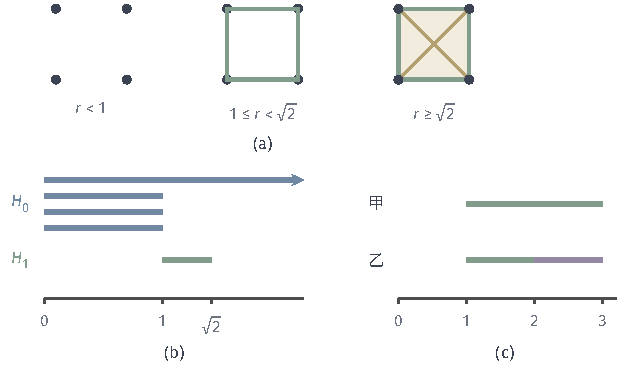
\includegraphics[width=105.346mm]{figures/04-spaces-measures-and-geometry/04-manifolds/tikz/mrec-filtration/figure.pdf}
  \caption{过滤与条形码。(a) 单位正方形的Rips过滤的三个阶段，浅黄表示填充的单纯形。(b) 正方形的条形码，蓝条是$H_0$（一根永不消失），绿条是$H_1$。(c) 过滤甲与过滤乙的$H_1$：逐尺度的Betti数相同，甲是一根贯穿的条，乙是前后相接的两根（绿、紫）。}
  \label{fig:mrec-filtration}
\end{BookInlineFigure}

\subsection{区间分解}
\label{sec:mrec-interval-decomposition}

持久模看起来是一串空间和映射，结构复杂。对有限点产生的过滤，它其实可以完全拆成最简单的块，每一块描述一个同调类从出现到消失的区间。

\paragraph{区间模与分解定理}

固定同调次数$k$。设$b<d\leq+\infty$，\term{区间模}（interval module）$I[b,d)$在$r\in[b,d)$处取$\mathbb R$，其余处取零空间；当$r\leq r'$都在$[b,d)$中时，映射是恒等映射，其余映射为零。它描述的正是一个在尺度$b$出现、在尺度$d$消失的同调类。

\begin{theorem}[区间分解]
\label{thm:mrec-interval-decomposition}
设过滤$\{K_r\}$由有限个复形组成，只在有限个尺度上变化，每个$K_r$都是有限复形。则对每个$k$，持久模$\{H_k(K_r),f_{r,r'}\}$同构于有限个区间模的直和$\bigoplus_lI[b_l,d_l)$，并且区间的多重集合$\{[b_l,d_l)\}$由持久模唯一确定。
\end{theorem}

证明要在所有尺度上同时选取相容的基，用到有限维空间中两个子空间族存在公共基的引理，篇幅较长，读者可查阅Zomorodian与Carlsson关于持久同调计算的论文。

结论的含义可以这样理解。可以在所有尺度上选取相容的基，使每个诱导映射都把基向量送到基向量或零。一个基向量对应一个区间，它出现的尺度是左端点，被送到零的尺度是右端点。这就像把线性映射化成对角形，只不过这里是一整串映射同时化简。两个分支合并时，约定保留出现较早的那个，较晚的那个记为消失，这一约定保证了分解的一致性。

由分解立刻得到一个常用的计数：$r\leq r'$时，$f_{r,r'}$的秩等于同时包含$r$和$r'$的区间的个数。

\paragraph{条形码与持久图}

区间的多重集合称为\term{条形码}（barcode），每个区间画成一根横条。也可以把每个区间$[b,d)$画成平面上的点$(b,d)$，分别称为出生坐标与死亡坐标，得到\term{持久图}（persistence diagram）；所有点都在对角线$b=d$上方，$d=+\infty$的点画在顶端。

端点的约定要说清。Rips过滤用闭条件，区间取左闭右开：类在尺度$b$已经存在，在尺度$d$恰好变为零或并入更早的类。Čech过滤用开球，单纯形在$r$严格超过阈值时才出现，区间实际是左开右闭的$(b,d]$，这只影响端点本身，不影响区间的长度和配对。不会在有限尺度消失的类对应$d=+\infty$，要保留在图中。

上一小节的例子可以直接读出条形码。正方形：$H_0$为$[0,\infty)$与三个$[0,1)$，$H_1$为$[1,\sqrt2)$。数轴上的三点：$H_0$为$[0,\infty)$、$[0,1)$、$[0,2)$。过滤甲的$H_1$为$[1,3)$，过滤乙的$H_1$为$[1,2)$与$[2,3)$，两者的区别清楚地显示出来，如图~\ref{fig:mrec-filtration}(b)(c)。

正六边形给出一个更有启发的比较。Rips过滤在$r=1$时出现六边形的环；$r=\sqrt3$时加入隔一个顶点的边，八个三角形恰好围成八面体的表面，环被填上，同时出现一个二维的空腔；$r=2$时加入对径的边，复形成为实心单纯形，空腔消失。所以$H_1$为$[1,\sqrt3)$，$H_2$为$[\sqrt3,2)$，见图~\ref{fig:mrec-barcodes}(a)。

Čech过滤的情形不同。由神经引理，它与平面中的球并同伦等价，而平面开集没有二维同调，所以没有$H_2$的条，$H_1$只有$(\tfrac12,1]$，见图~\ref{fig:mrec-barcodes}(b)。Rips过滤多出来的那根$H_2$条，正是它“成对相交就算有公共点”造成的，并不反映任何真实的二维结构。

条形码是跨尺度同调的表示，它不记录点的坐标，也不记录同胚类型或光滑结构。两组完全不同的点可以有相同的条形码，例如把整组点作任意合同变换，Rips过滤不变。

\begin{BookInlineFigure}
  \centering
  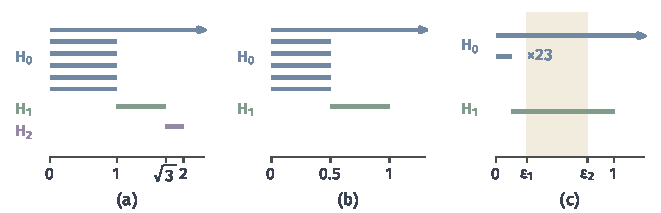
\includegraphics[width=112mm]{figures/04-spaces-measures-and-geometry/04-manifolds/matplotlib/mrec-barcodes/figure.pdf}
  \caption{由边界矩阵算出的条形码，横轴为尺度。(a) 单位正六边形的Rips过滤，$H_2$的条是八面体空腔。(b) 同一组点的Čech过滤，横轴为球半径，没有$H_2$。(c) 单位圆上$24$个等距样本的Čech过滤，$H_0$有$23$根相同的短条，$H_1$的唯一长条横跨浅黄色的恢复窗口$(\varepsilon_1,\varepsilon_2)$。}
  \label{fig:mrec-barcodes}
\end{BookInlineFigure}

\subsection{瓶颈距离}
\label{sec:mrec-bottleneck}

要谈条形码的稳定性，先要能比较两张持久图。数据稍有变化，长条的端点应该稍有移动，同时可能冒出或消失一些很短的条。比较时应把长条与长条配对，短条则允许与“无”配对，代价是它本身的长度。

\begin{definition}[瓶颈距离]
\label{def:mrec-bottleneck}
固定同调次数，设$D_1,D_2$是两张持久图，即点$(b,d)$的有限多重集合。部分匹配是$D_1$与$D_2$之间的一个部分双射，未被匹配的点改为与对角线匹配。匹配的点对$(b,d)$与$(b',d')$的代价为$\max(\lvert b-b'\rvert,\lvert d-d'\rvert)$，与对角线匹配的点$(b,d)$的代价为$(d-b)/2$。\term{瓶颈距离}（bottleneck distance）$d_B(D_1,D_2)$是全部部分匹配中最大代价的最小值。
\end{definition}

点$(b,d)$到对角线的$L^\infty$距离恰为$(d-b)/2$，所以与对角线匹配就是把点移到最近的对角线位置，如图~\ref{fig:mrec-diagram}(a)。死亡坐标为$+\infty$的点，只能与死亡坐标同为$+\infty$的点匹配，代价取$\lvert b-b'\rvert$；两张图中这类点个数不同时，瓶颈距离为$+\infty$。

\begin{example}[两张一维持久图]
\label{ex:mrec-bottleneck}
考虑下面两张持久图：
\[
 D_1=\{(1,3)\},\qquad D_2=\{(1.2,2.9),\ (2,2.2)\}.
\]
把$(1,3)$与$(1.2,2.9)$匹配，代价是
\[
 \max(0.2,\ 0.1)=0.2 .
\]
把$(2,2.2)$与对角线匹配，代价是$0.1$。最大代价为$0.2$，所以$d_B\leq0.2$。

反过来，任何匹配中$(1,3)$都要有去处：与$(1.2,2.9)$匹配代价$0.2$，与$(2,2.2)$匹配代价$\max(1,0.8)=1$，与对角线匹配代价$1$。所以最大代价至少为$0.2$，于是
\[
 d_B(D_1,D_2)=0.2 .
\]
短条$(2,2.2)$只贡献了$0.1$，它的出现几乎不改变距离。
\end{example}

\begin{BookInlineFigure}
  \centering
  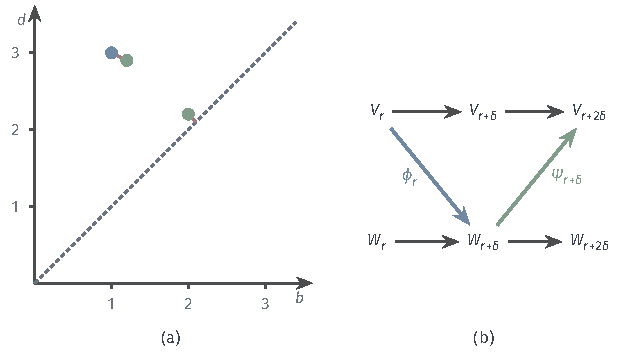
\includegraphics[width=105.184mm]{figures/04-spaces-measures-and-geometry/04-manifolds/tikz/mrec-diagram/figure.pdf}
  \caption{持久图的匹配与持久模的交错。(a) 例~\ref{ex:mrec-bottleneck}的两张持久图，$D_1$为蓝点，$D_2$为绿点，红色线段表示最优匹配，靠近对角线的绿点匹配到对角线。(b) 交错的一个片段：先走蓝色的$\phi$，再走绿色的$\psi$，结果等于沿$V$直接走$2\delta$。}
  \label{fig:mrec-diagram}
\end{BookInlineFigure}

\subsection{过滤交错}
\label{sec:mrec-interleaving}

现在比较同一组点标签上的两张距离表。设$d=[d_{i,j}]$与$d'=[d'_{i,j}]$都是对称、零对角的非负矩阵，可以来自同一组点在两次测量中的结果，并且$\lvert d_{i,j}-d'_{i,j}\rvert\leq\delta$对所有$i,j$成立。记$R_r(d)$为按距离表$d$、直径界$r$构造的Rips复形。

若$\sigma$在$R_r(d)$中，它的每对顶点满足$d_{i,j}\leq r$，从而$d'_{i,j}\leq r+\delta$，所以$\sigma$在$R_{r+\delta}(d')$中。对称地，$R_r(d')\subseteq R_{r+\delta}(d)$。于是两套过滤交替地相互包含：
\begin{equation}
 R_r(d)\subseteq R_{r+\delta}(d')\subseteq R_{r+2\delta}(d),
 \label{eq:mrec-rips-interleave-1}
\end{equation}
\begin{equation}
 R_r(d')\subseteq R_{r+\delta}(d)\subseteq R_{r+2\delta}(d').
 \label{eq:mrec-rips-interleave-2}
\end{equation}

这些复形都是同一个顶点集上全体单纯形的子复形，所有映射都是包含，所以复合的包含$R_r(d)\subseteq R_{r+2\delta}(d)$与原过滤中的推进是同一个包含，与沿过滤推进再平移的各种路径都相容。把这种“隔一步能互相换过去、并且与自身的推进相容”的关系抽象出来，就是下面的定义。

\begin{definition}[交错]
\label{def:mrec-interleaving}
设$\{V_r,v_{r,r'}\}$与$\{W_r,w_{r,r'}\}$是两个持久模，$\delta\geq0$。若存在线性映射$\phi_r:V_r\to W_{r+\delta}$与$\psi_r:W_r\to V_{r+\delta}$，它们与两个持久模自身的映射交换，并满足$\psi_{r+\delta}\circ\phi_r=v_{r,r+2\delta}$与$\phi_{r+\delta}\circ\psi_r=w_{r,r+2\delta}$，则称两个持久模$\delta$\term{交错}（interleaved）。
\end{definition}

图~\ref{fig:mrec-diagram}(b)画的是其中一个等式：沿蓝、绿两条斜线走到$V_{r+2\delta}$，与沿上面一行直接走是同一个映射。对两套Rips过滤取$k$维同调，式~\eqref{eq:mrec-rips-interleave-1}和式~\eqref{eq:mrec-rips-interleave-2}的包含诱导出$\phi_r$与$\psi_r$；包含的复合等于包含，诱导映射的复合也就等于诱导映射，定义中的等式全部成立。所以两个持久模$\delta$交错。

交错为什么能控制条形码？下面的不等式给出最直接的一步。

\begin{lemma}[秩的比较]
\label{lem:mrec-rank-interleaving}
设两个持久模$\delta$交错，$r+2\delta\leq r'$，则
\begin{equation}
 \operatorname{rank}v_{r,r'}\leq\operatorname{rank}w_{r+\delta,r'-\delta}.
 \label{eq:mrec-rank-interleaving}
\end{equation}
\end{lemma}
\begin{proof}
由交错的定义，$v_{r,r'}$可以分解为
\[
 V_r\xrightarrow{\ \phi_r\ }W_{r+\delta}\xrightarrow{\ w\ }W_{r'-\delta}\xrightarrow{\ \psi_{r'-\delta}\ }V_{r'} .
\]
事实上，$\phi$与两个持久模自身的映射交换，所以
\[
 w_{r+\delta,r'-\delta}\circ\phi_r=\phi_{r'-2\delta}\circ v_{r,r'-2\delta}.
\]
再用交错定义中的等式，
\[
 \psi_{r'-\delta}\circ\phi_{r'-2\delta}=v_{r'-2\delta,r'} ,
\]
就得到$v_{r,r'}$。复合映射的秩不超过中间映射的秩。
\end{proof}

由区间分解后的计数，式~\eqref{eq:mrec-rank-interleaving}说：$V$中覆盖$[r,r']$的条的根数，不超过$W$中覆盖$[r+\delta,r'-\delta]$的条的根数。这正是“一根条在对方那里有一根端点相差不超过$\delta$的对应条”的计数形式。把这些计数不等式对所有$r,r'$合起来，再用组合匹配的论证，就能得到下面的定理。

\begin{theorem}[持久图的稳定性]
\label{thm:mrec-stability}
设两个持久模的每个空间都是有限维的，并且它们$\delta$交错，则它们的持久图的瓶颈距离不超过$\delta$。特别地，若两张距离表逐项之差不超过$\delta$，则对每个$k$，两套Rips过滤的$k$维持久图满足$d_B\leq\delta$。
\end{theorem}

这一结果称为代数稳定性定理，从计数不等式到匹配的证明较长，读者可查阅Chazal等人关于持久模稳定性的论文。

它的作用是把几何上的扰动换成表示上的扰动。例如每个点移动不超过$\eta$，成对距离至多改变$2\eta$，持久图在瓶颈距离下至多移动$2\eta$。长于$4\eta$的条不会因此消失，只是端点稍有移动；短于这个量的条则可能出现或消失。

定理控制的只是表示的变化。它说两次测量得到的持久图相近，却没有说任何一张持久图反映了底层流形的同调：两张距离表都可能来自采样不足的数据，它们的条形码彼此接近，同时都与流形无关。

\subsection{持久信息的解释}
\label{sec:mrec-persistence-interpretation}

把持久同调与第~\ref{sec:mrec-homology-recovery}节的恢复定理放在一起，可以分清哪些结论有保证。设样本$P\subseteq M$的覆盖精度$\delta_P$满足
\begin{equation}
 2\delta_P<\varepsilon_1<\varepsilon_2<\sqrt{3/5}\,\tau ,
 \label{eq:mrec-recovery-window}
\end{equation}
则区间$[\varepsilon_1,\varepsilon_2]$中的每个$\varepsilon$都满足定理~\ref{thm:mrec-homology-recovery}的条件，称它为恢复窗口。

\paragraph{窗口内的条}

对窗口中的$\varepsilon\leq\varepsilon'$，包含$j:U_\varepsilon\hookrightarrow U_{\varepsilon'}$是同伦等价。理由如下：记$i:M\hookrightarrow U_\varepsilon$、$i':M\hookrightarrow U_{\varepsilon'}$，二者都是同伦等价，且$j\circ i=i'$；取$i$的同伦逆$h$，则
\[
 j\simeq j\circ i\circ h=i'\circ h,
\]
是同伦等价的复合。所以$H_k(U_\varepsilon)\to H_k(U_{\varepsilon'})$是同构。

进一步可以证明，神经引理中的同伦等价能与包含相容地选取，这要求把神经引理的证明做成对包含自然的形式，读者可查阅Chazal与Oudot关于持久性重建的论文。于是Čech过滤在窗口内的诱导映射都是同构。由区间分解，没有区间的端点落在窗口内部，凡是与窗口相交的条都横跨整个窗口，并且这样的$k$维条恰有$\beta_k(M)$根。这是已经建立了恢复保证的结论。

单位圆上$24$个等距样本的例子可以把这件事算到底。条件给出窗口$\varepsilon_1=2\delta_P\approx0.262$到$\varepsilon_2\approx0.775$。Čech过滤中，相邻两球在$r$超过弦长的一半$\approx0.131$时相交，圆环在此形成；圆心在$r$超过$1$时才被覆盖。所以$H_1$唯一的条是$(0.131,1]$，它横跨窗口，根数$1=\beta_1(S^1)$；$H_0$除了永不消失的条，$23$根短条都在$0.131$处结束，在窗口之前，见图~\ref{fig:mrec-barcodes}(c)。

\paragraph{窗口外的条}

窗口外的条没有这样的保证。很靠近$0$的短条通常反映采样的离散性，很大尺度上的条则反映样本整体的粗略形状，它们与$M$的关系都没有经过论证。更重要的是，实际中并不知道$\delta_P$和$\tau$，也就不知道窗口在哪里，甚至不知道窗口是否存在。

没有覆盖、噪声和几何尺度的条件时，寿命长只表示同调类跨越很大的尺度范围而持续存在。一个例子是：底层集合是一个实心圆盘，没有洞，但样本只取在它的边界圆附近。Rips过滤会给出一根很长的一维条，它如实地反映了样本的形状，却不是圆盘的孔洞；问题出在样本没有覆盖圆盘内部，任何对持久图的处理都无法补上未被采样的区域。

\paragraph{其他过滤与噪声}

上面的结论是对样本在流形上的Čech过滤建立的。对Rips过滤，只能借助式~\eqref{eq:mrec-cech-rips}的夹逼关系，把恢复窗口中的信息传过来，这要求窗口跨越一倍以上的尺度，需要另行论证；正六边形的$H_2$条提醒我们，Rips过滤确实可能给出流形中不存在的同调。观测离开流形时，恢复窗口本身需要重新建立。

表示的稳定性也不能单独证明真实孔洞的存在：定理~\ref{thm:mrec-stability}保证小扰动不会让长条消失，但长条从哪里来，要由覆盖、噪声和可达半径的条件回答。持久同调提供的是跨尺度的完整记录及其稳定性，它与恢复保证配合使用，不能替代后者。
